\documentclass{beamer}
\setbeamertemplate{bibliography item}{\insertbiblabel}
\usepackage[frenchb]{babel}
\usepackage[T1]{fontenc}
\usepackage[utf8]{inputenc}
\usepackage{wrapfig}
\usepackage{color}
\usepackage{graphicx}
\usepackage{tikz}
\usepackage{bbm}

\DeclareMathOperator*{\argmax}{argmax}
\DeclareMathOperator*{\argmin}{argmin}

\usetheme{Berlin}


\title{Robot's perception in natural interaction skills learning}

\author{Bozorgmehr Aminian}

\institute{Idiap}

\date{August, 2018}


\setbeamertemplate{footline}[frame number] 


\begin{document}


\begin{frame}

\titlepage

\end{frame}

\begin{frame}
\tableofcontents
\end{frame}

\section{Introduction}


\subsection{Motivation}
\begin{frame}
\textbf{Provides the required measurements about}:
\begin{itemize}
\item People
\item Scene object
\item Gestures
\item Verbal and non-verbal communication
\end{itemize}
\begin{center}
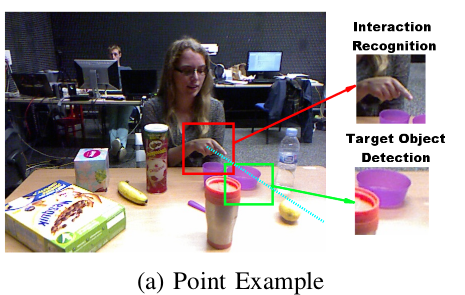
\includegraphics[scale=0.3]{Pictures/ActionRecognition1.png}
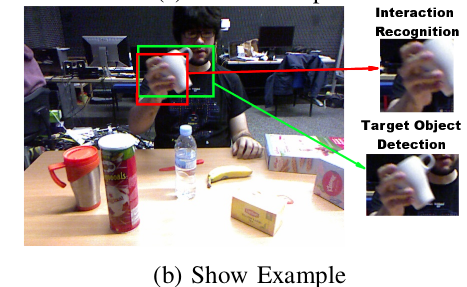
\includegraphics[scale=0.3]{Pictures/ActionRecognition2.png}
\end{center}
\end{frame}

\begin{frame}
\textbf{Understanding of the teacher's natural behavior}:
\begin{itemize}
\item Segmentation (start, end, reference-action sequence)
\item Attention (person/object of interest)
\item Feedback (positive/negative, interruption)
\end{itemize}
\begin{center}
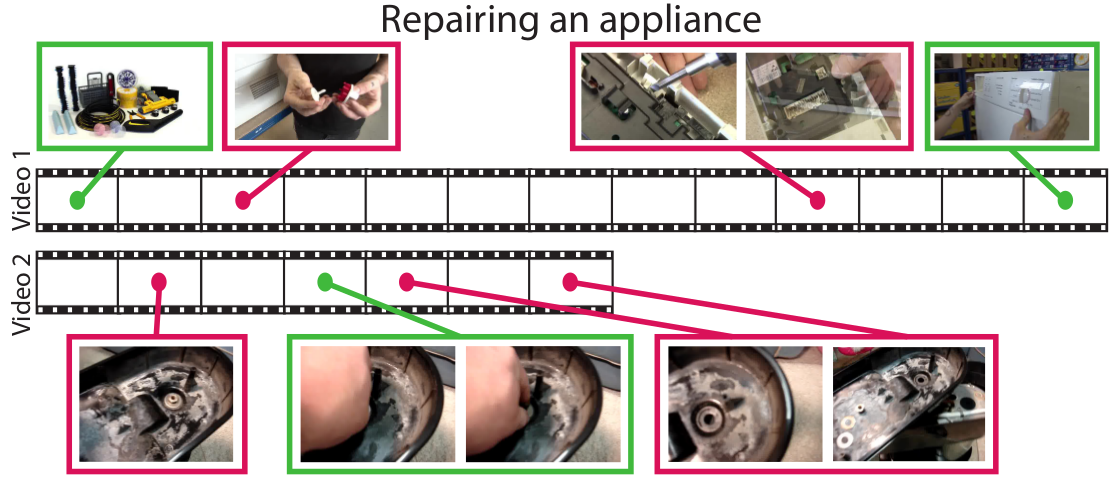
\includegraphics[scale=0.2]{Pictures/ActionSegmentation.png} \\
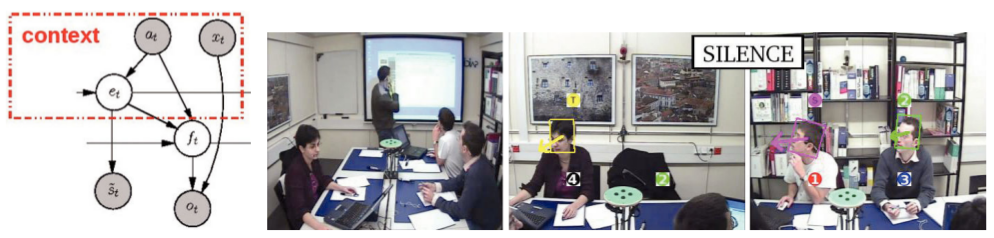
\includegraphics[scale=0.25]{Pictures/SceneRepresentation.png}
\end{center}
\end{frame}

\begin{frame}
\textbf{Use sensors in a every day's life framework (natural behavior)}:
\begin{itemize}
\item RGB camera
\item Depth sensor (kinect v2)
\item Microphone
\end{itemize}
\begin{center}
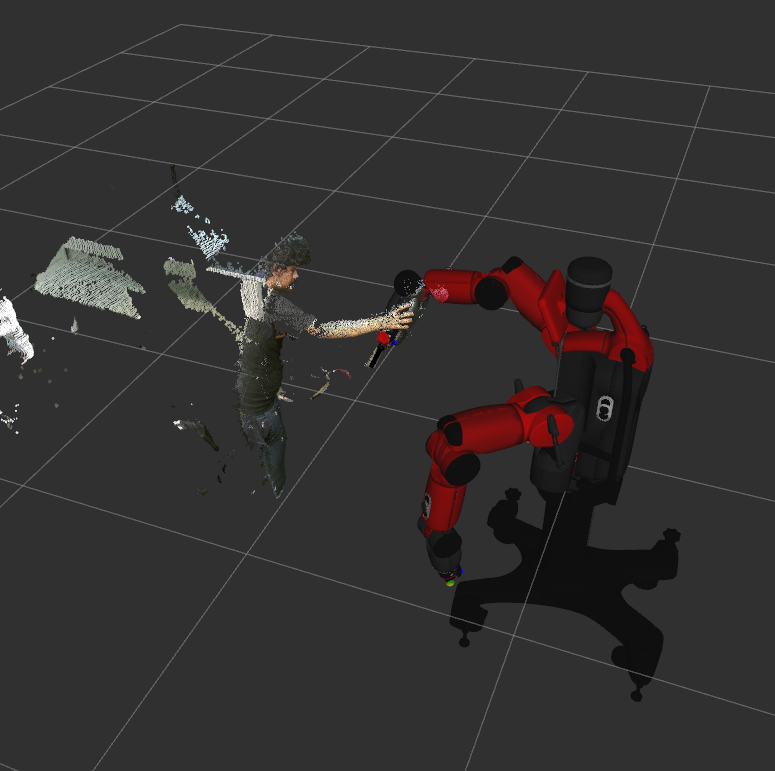
\includegraphics[scale=0.2]{Pictures/KinectRobotImage.png} \\
\end{center}
\end{frame}

\subsection{Approach}

\begin{frame}
\textbf{Gaze tracking and attention modeling}:
\begin{itemize}
\item Unsupervised gaze calibration
\begin{itemize}
\item Head tracker (3DMM, ICP).
\item Gaze tracker (G3E, kNN, H-SVR, R-SVR).
\item Gaze calibration (interaction prior based, LSMed).
\end{itemize}
\item Contextual interaction models for gaze activity interpretation (VFOA)
\end{itemize}
\begin{center}
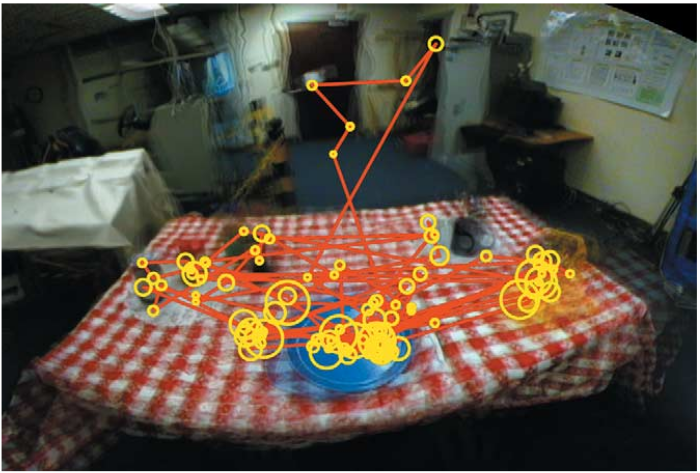
\includegraphics[scale=0.2]{Pictures/VFOA_Sandwich.png} \hspace{0.5cm}
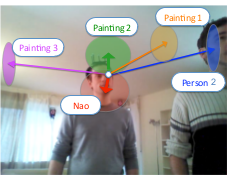
\includegraphics[scale=0.55]{Pictures/VFOA_Vernissage.png}
\end{center}
\end{frame}

\section{Gaze Tracker}
\begin{frame}
\textbf{Gaze Tracker}
\begin{center}
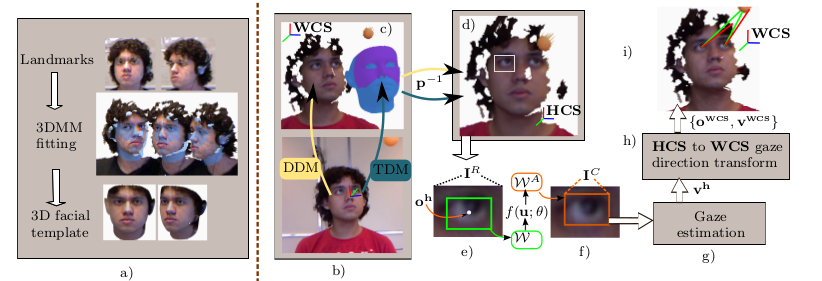
\includegraphics[scale=0.4]{Pictures/HG3D_bis.png}
\end{center}
\end{frame}

\begin{frame}
\textbf{Gaze Tracker}
\begin{center}
Wrong Head pose ~~ Correct Head pose \\
$\Rightarrow$ Wrong cropping ~~$\Rightarrow$ Correct cropping \\
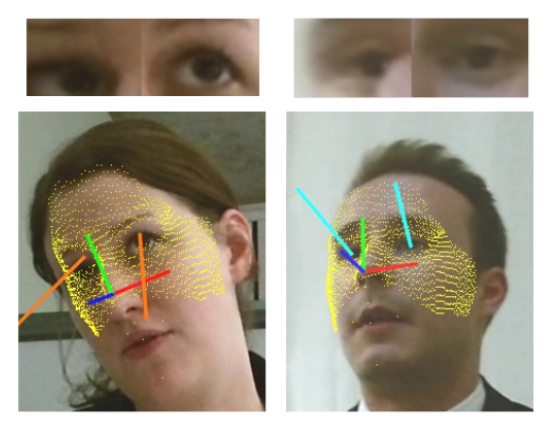
\includegraphics[scale=0.3]{Pictures/EyeCropping.png} \\
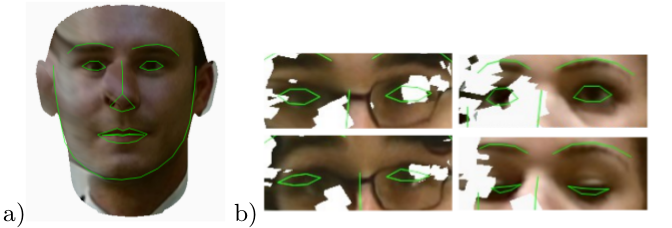
\includegraphics[scale=0.2]{Pictures/LandmarkEye.png}
\end{center}
\end{frame}


\subsection{Data}

\begin{frame}
\textbf{Head Pose}: \newline
Rotation matrix $R_t \in SO(3)$ , $T_t \in \mathbb{R}^3$ vector at time $t\in \mathbb{R}$. The head pose is defined by
\begin{equation}
p_t := (R_t, T_t)
\end{equation}
\begin{center}
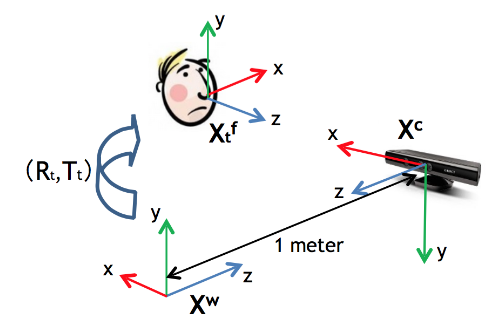
\includegraphics[scale=0.18]{Pictures/HeadPoseWCS.png}
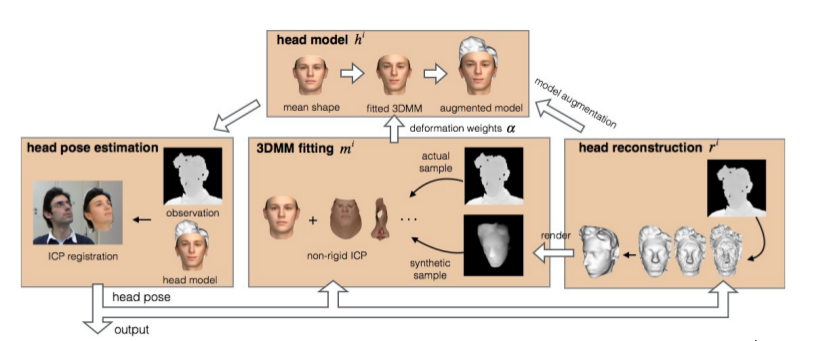
\includegraphics[scale=0.27]{Pictures/HeadPose.png}
\end{center}
\end{frame}

\begin{frame}
\textbf{Eye Center}: \newline
Coordinate of the eye center $o_t \in \mathbb{R}^3$.
\vspace{0.5cm}

\textbf{Gaze Direction}: \newline 
Tilt angle $\phi_t \in [-\pi/2,\pi/2]$ and pan angle $\theta_t \in [-\pi/2,\pi/2]$ at time $t$ in a \textit{head coordinate system}. The gaze direction is defined by 
\begin{equation}
g_t = (\phi_t,\theta_t)
\end{equation}
\begin{center}
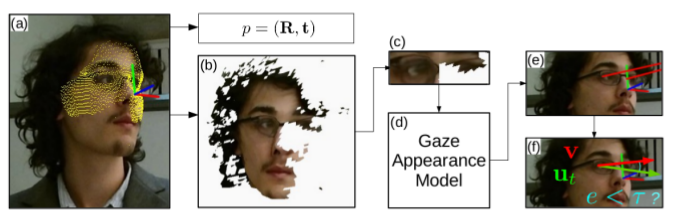
\includegraphics[scale=0.4]{Pictures/HG3D.png}
\end{center}
\end{frame}

\begin{frame}
\textbf{Unitary Gaze Direction Vector}: \newline
There exists a mapping $\Phi: \mathbb{R}^2 \rightarrow \mathbb{R}^3$ such that the unitary gaze direction vector is given by
\begin{equation}
\Phi(g_t) = v_t,~\forall t \in \mathbb{R}.
\end{equation}
\textbf{Ground Truth}: \newline
For an object coordinate $x \in \mathbb{R}^3$. The ground truth is defined by 
\begin{equation}
\bar{v}_t = \frac{x-o_t}{\|x-o_t\|}~\text{and}~\bar{g}_t = \Phi^{-1}(\bar{v}_t)
\end{equation}
\end{frame}

\subsection{Calibration}

\begin{frame}
\textbf{Gaze Calibration} \newline
For a set of parameters $\alpha= \{\alpha_1,..., \alpha_k \}$. The gaze calibration consists in the optimization problem
\begin{equation}
\text{minimize}~ \|G(p_t,g_t; \alpha) - \bar{g}_t \| ~ \text{for} ~ t \in \mathbb{R}.
\end{equation}
\begin{center}
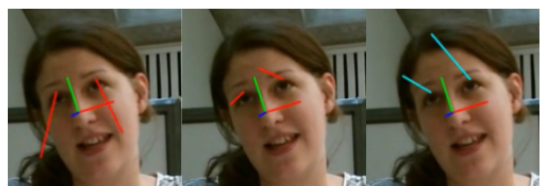
\includegraphics[scale=0.4]{Pictures/GazeCalibration.png} \\
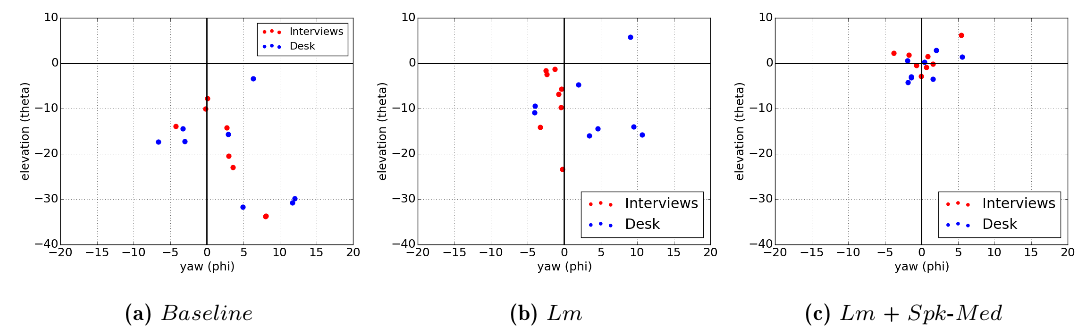
\includegraphics[scale=0.25]{Pictures/GazeCalibrationGraph.png} 
\end{center}
\end{frame}

\section{Robot}

\subsection{Setup}

\begin{frame}
\textbf{Gaze Calibration Experiment}:
\begin{center}
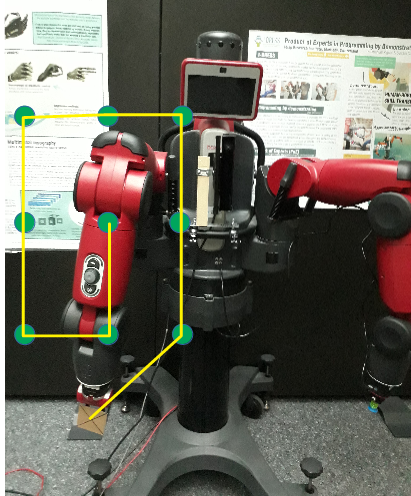
\includegraphics[scale=0.4]{Pictures/Baxter_Setup_Dynamic.png} \hspace{0.5cm}
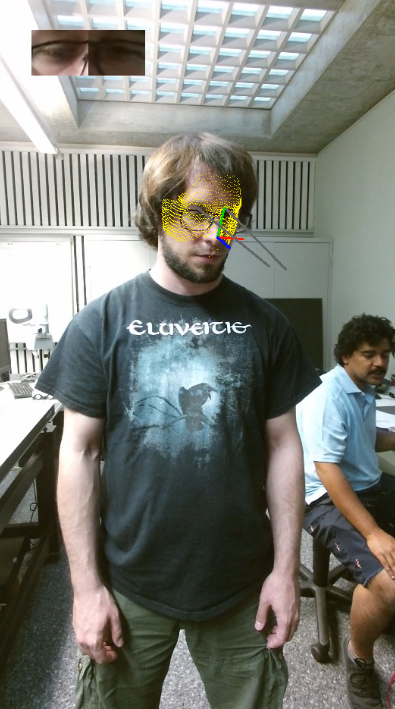
\includegraphics[scale=0.3]{Pictures/Baxter_View.png}
\end{center}
\end{frame}

\subsection{Kinematics}

\begin{frame}
\textbf{Forward kinematics}: \newline
For $\theta \in \mathbb{R}^{k}$, define $X: \mathbb{R}^k \rightarrow \mathbb{R}^{n}$ such that 
\begin{equation}
X = X(\theta).
\end{equation}
\textbf{Inverse kinematics}: \newline
For $Y \in \mathbb{R}^{n}$, find $\theta \in \mathbb{R}^{k}$ such that
\begin{equation}
X(\theta) - Y = 0
\end{equation}
\end{frame}

\begin{frame}
\begin{itemize}
\item Cost function:
\begin{equation}
E(\theta) = \frac{1}{2} \| X(\theta) - Y\|^2
\end{equation}
\item Gradient:
\begin{align*}
\frac{\partial E}{\partial \theta}(\theta) &= (X(\theta) - Y)^T\frac{\partial X}{\partial \theta}(\theta) \\
 & = (X(\theta) - Y)^T J \\
 & =: d\theta
\end{align*}
\item Update rule
\begin{equation}
\theta^{m+1} = \theta^m - \eta d\theta^m
\end{equation}
\end{itemize}
\end{frame}

\begin{frame}
\begin{itemize}
\item Constraints:
\begin{equation}
\theta^- \, \preceq  \, \theta  \, \preceq  \, \theta^+
\end{equation}
\item Indicator: for $i=1,...,k$,
\begin{equation}
[\text{Idc}(\theta)]_i = \mathbbm{1}_{\{ \theta^-_i \leq \theta_i \leq \theta^+_i \}^c} = \left\{
\begin{array}{ll}
0 &~\text{if}~ \theta^-_i \leq \theta_i \leq \theta^+_i, \\
1 &~\text{otherwise}.
\end{array}
\right.
\end{equation}
\item Update rule (identity matrix $I_k \in \mathbb{R}^{k \times k}$)
\begin{equation}
\theta^{m+1} = \theta^m - (\eta I_k - \lambda \text{diag}(\text{Idc}(\theta^m))) d\theta^m, ~ \lambda \geq \eta.
\end{equation}
\end{itemize}
\end{frame}

\section{Camera}

\subsection{Intrinsic}
\begin{frame}
\textbf{Camera rotation}:
\begin{center}
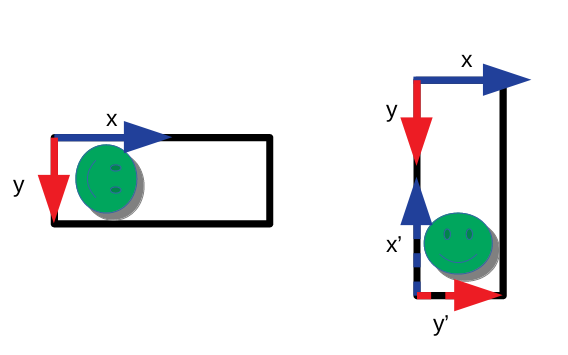
\includegraphics[scale=0.3]{Pictures/CameraVerticalRotation.png}
\end{center}
\begin{equation}
x' = -y ~\text{and}~ y' = x
\end{equation}
Hence
\begin{equation}
P = \left(
\begin{array}{ccc}
0 & 1 & 0 \\
-1 & 0 & 0 \\
0 & 0 & 1
\end{array}
\right)
\end{equation}
\end{frame}

\begin{frame}
\textbf{Camera intrinsic}:
\begin{itemize}
\item Camera matrix:
\begin{equation}
K = \left(
\begin{array}{ccc}
f_x & 0 & c_x \\
0 & f_y & c_y \\
0 & 0 & 1
\end{array}
\right).
\end{equation}
\item 
After rotation:
\begin{equation}
K' = \left(
\begin{array}{ccc}
f_y & 0 & c_y \\
0 & f_x & s_x - c_x \\
0 & 0 & 1
\end{array}
\right) 
\end{equation}
where $(s_x,s_y)$ is the size of the original image.
\end{itemize}
\end{frame}

\subsection{Extrinsic}

\begin{frame}
\textbf{Camera extrinsic}:
\begin{center}
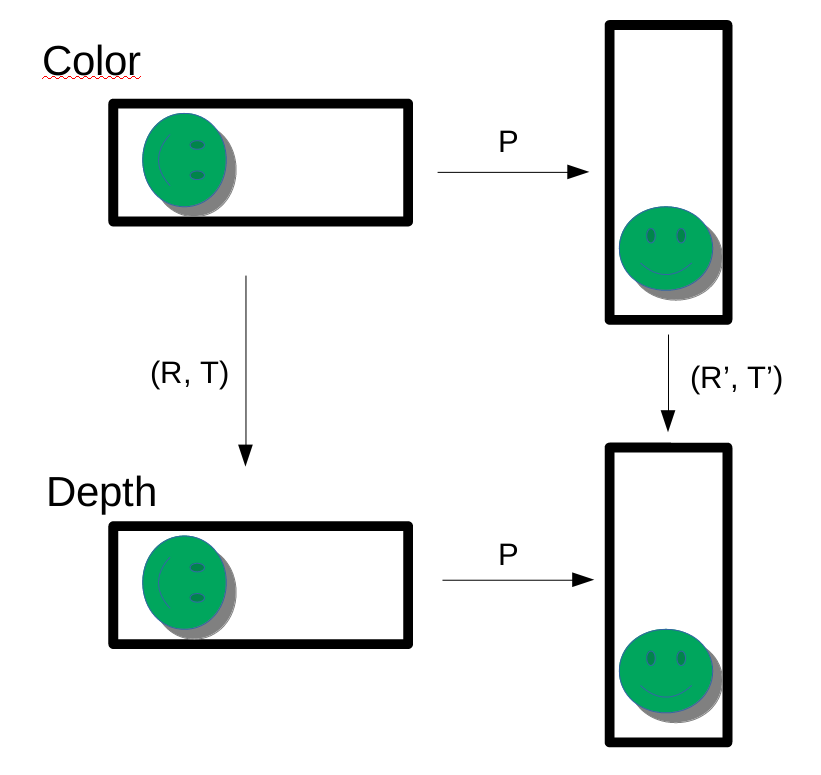
\includegraphics[scale=0.2]{Pictures/CameraExtrinsicRotation.png}
\end{center}
\begin{equation}
R' = PRP^{-1}~ \text{and}~ T' = PT
\end{equation}
\end{frame}

\section{Robot and Camera}

\subsection{Calibration}

\begin{frame}
\textbf{Robot-camera calibration}
\begin{center}
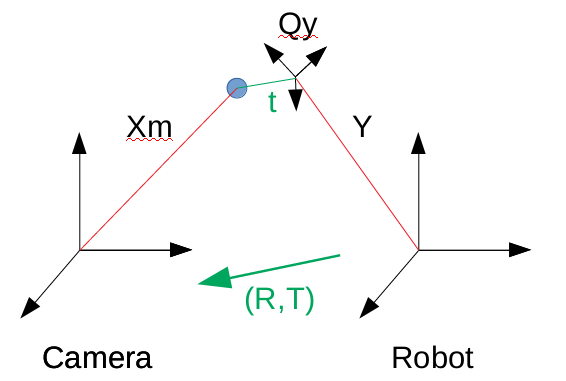
\includegraphics[scale=0.5]{Pictures/RobotCameraCalibrationFrame.png}
\end{center}
\end{frame}

\begin{frame}
\begin{itemize}
\item $\mathcal{F}_X$ ~$\mathcal{F}_Y$: camera frame, resp. robot frame. 
\item $X$, $Y$: coordinate of the end-effector in $\mathcal{F}_X$, resp. in $\mathcal{F}_Y$.
\item $X_m$ $Y_m$: coordinate of the marker in $\mathcal{F}_X$, resp. in $\mathcal{F}_Y$.
\item $\mathcal{F}_{Q_Y}$: end-effector frame.
\item $t$: coordinate of the marker in $\mathcal{F}_{Q_Y}$.
\item $Q_Y \in \mathbb{R}^{3 \times 3}$: basis vector of the frame $\mathcal{F}_{Q_Y}$ expressed in frame $\mathcal{F}_Y$. It corresponds to the rotation matrix from $\mathcal{F}_{Y}$  to $\mathcal{F}_{Q_Y}$. 
\end{itemize}
\end{frame}

\begin{frame}
\begin{itemize}
\item Known data ($n$ images): $X_m= \{X_m^i\}_{i=1}^n$, $Y= \{Y^i\}_{i=1}^n$ and $Q_Y= \{Q_Y^i\}_{i=1}^n$.
\item Unknowns: rigid transform $(R, T)$ from $\mathcal{F}_Y$ to $\mathcal{F}_X$ and vector $t\in \mathbb{R}^{3}$:
\begin{equation}
R Y + T = X ~ \text{and} ~ R Y_m + T = X_m
\end{equation}
\item Remark: 
\begin{itemize}
\item $R = R_{\gamma}R_{\beta}R_{\alpha}$ where $(\alpha, \beta, \gamma)$ are Euler angles.
\item $Q_Y = Q_Y(q_Y)$ where $q_Y$ is the quaternion coordinates of the orientation of the end-effector   in $\mathcal{F}_Y$.
\end{itemize}
\end{itemize}
\end{frame}

\begin{frame}
\begin{itemize}
\item Solve for images $i=1,...,n$ :
\begin{equation}
R \left( Y^i + Q_Y^i t \right) + T = X_m^i
\end{equation}
\item Substract mean:
\begin{equation}
R \left( \bar{Y}^i + \bar{Q}_Y^i t \right) = \bar{X}_m^i
\end{equation}
where
\begin{equation*}
\bar{Y}^i = \left(Y^i - \frac{1}{n}\sum_{k=1}^n Y^i \right),~\bar{Q}_Y^i = \left(Q_Y^i - \frac{1}{n}\sum_{k=1}^n Q_Y^i\right) 
\end{equation*}
\begin{equation*}
\bar{X}_m^i =\left(X_m^i - \frac{1}{n}\sum_{k=1}^n X_m^i\right)
\end{equation*}
\item Cost function:
\begin{equation}
E(\alpha, \beta, \gamma, t) = \frac{1}{2} \sum_{i=1}^n \left\| R \left( \bar{Y}^i + \bar{Q}_Y^i t \right) - \bar{X}_m^i \right\|^2
\end{equation}
\end{itemize}
\end{frame}

\begin{frame}
\textbf{Procrustes problem}: \newline
For $X,\, Y \in \mathbb{R}^{3 \times N}$
\begin{equation}
R = \argmin_{\Omega} \| \Omega X -Y \|~\text{subject to}~ \Omega^T\Omega = I
\end{equation}
\textbf{Procrustes solution}: \newline
For $M := Y X^T = U \Sigma V^T$ a singular value decomposition (SVD), then
\begin{equation}
R = U V^T .
\end{equation}
\end{frame}

\subsection{Synchronization}

\begin{frame}
\textbf{Synchronize robot and camera time}:
\begin{itemize}
\item Robot has its own time.
\item Camera's time is computer time (- latency)
\item Set robot's time to computer time (latency is small for robot topics).
\end{itemize}
\end{frame}

\section{Future Work}
\begin{frame}
Output of perception:
\begin{itemize}
\item Task
\begin{itemize}
\item Make a cup of tea (intelligent robot)
\item This is a cup (idiot robot but may improve!)
\item Take the cup in front. Take the kettle. Pour the cup.
\end{itemize}
\item Interraction
\begin{itemize}
\item What is a cup?
\item How to grasp it?
\item Where is the cup?
\item Non-verbal communication from the robot (gaze, legible motion)
\end{itemize}
\end{itemize}
\end{frame}

\begin{frame}
Input of perception:
\begin{itemize}
\item Object
\begin{itemize}
\item Detection (ID)
\item Recognition (name)
\item Position/Orientation
\item Affordance
\item Color
\item ...
\end{itemize}
\item Posture
\begin{itemize}
\item Tronc
\item Hands (and gesture)
\item Arms
\item Head pose
\end{itemize}
\item Verbal and non-verbal communication
\begin{itemize}
\item Speech
\item Gaze
\item Emotion
\end{itemize}
\end{itemize}
\end{frame}

\begin{frame}
Actual Work:
\begin{itemize}
\item Gaze classification (Rémy, 1 papers)
\item Gaze as prior for task recognition (2 papers)
\item Unsupervised gaze calibration
\item Design of experiment
\begin{itemize}
\item House benchmark
\item Work benchmark
\end{itemize}
\item Building machines that learn and think like people
\end{itemize}
\end{frame}


\end{document}